\chapter{Návrh vylepšení systému}
\DIFaddbegin \DIFadd{V této kapitole jsou navrženy způsoby vylepšení navrženého systému.
}\DIFaddend 


%%%%%%%%%%%%%%%%%%%%%%%%%%%%%%%%%%%%%%%%%%%%%%%%%%%%%%
\section{Návrh gatewaye verze 2}
Pro lepší mechanické uspořádání byla navržena verze 2 \DIFdelbegin \DIFdel{, kde je }\DIFdelend \DIFaddbegin \DIFadd{s navrženým plošným spojem (PCB).
Schéma zapojení je v obrázku \ref{fig:minigateway_schema} a plošný spoj je v obrázku \ref{fig:minigateway_plosnak}.
Je zde }\DIFaddend použit \DIFdelbegin \DIFdel{i }\DIFdelend jiný vývojový kit NUCLEO-L432KC s \DIFaddbegin \DIFadd{výkonnějšim }\DIFaddend procesorem STM32L432KC, který \DIFaddbegin \DIFadd{má pinout stejný jako Arduino Nano, tedy je pod tímto názvem ve shcématu.
LoRa transceiver je použit RFM95w \mbox{%DIFAUXCMD
\cite{RFM95w} }\hspace{0pt}%DIFAUXCMD
bez shieldu.
RS485 transceiver je použit LTC1480. 
Do zařízení }\DIFaddend je \DIFdelbegin \DIFdel{výkonnější.
Navíc je zde }\DIFdelend \DIFaddbegin \DIFadd{dále }\DIFaddend přidán externí stabilizátor, napěťový filtr, \DIFdelbegin \DIFdel{přepínačem }\DIFdelend \DIFaddbegin \DIFadd{přepínač }\DIFaddend volitelné impedanční zakončení sítě RS485 a \DIFdelbegin \DIFdel{proudové ochrany }\DIFdelend \DIFaddbegin \DIFadd{napěťové ochrany pro linky A, B a napájení}\DIFaddend . 

\begin{figure}[!h]
    \centering
    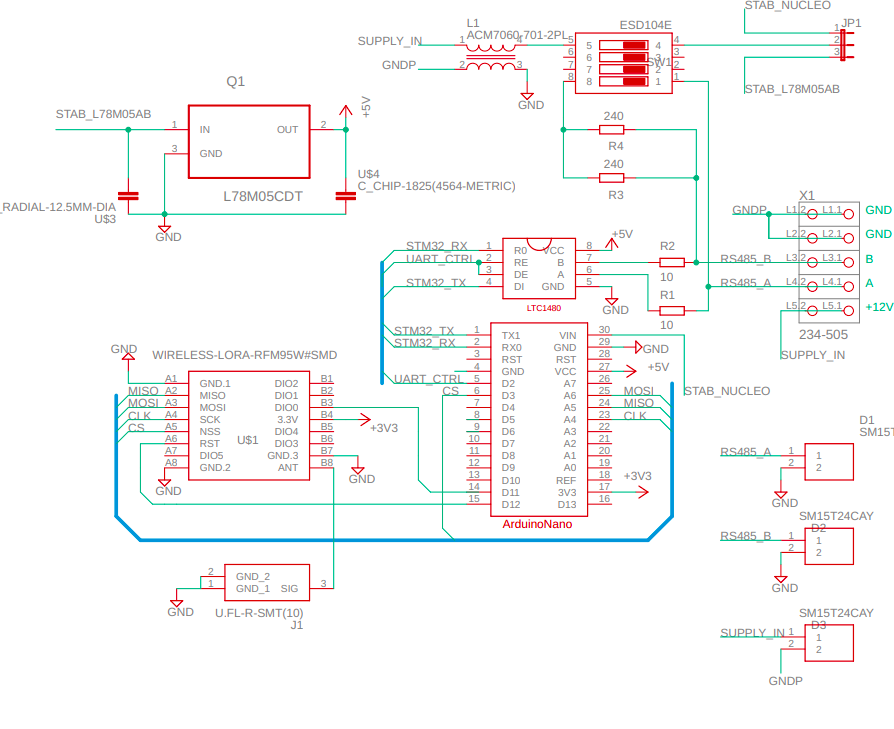
\includegraphics[width=1\textwidth]{minigateway_schema}
    \caption{Návrh \DIFdelbeginFL \DIFdelFL{WSN }\DIFdelendFL gatewaye verze 2 - schéma}
    \label{fig:minigateway_schema}
\end{figure}

\begin{figure}[!h]
    \centering
    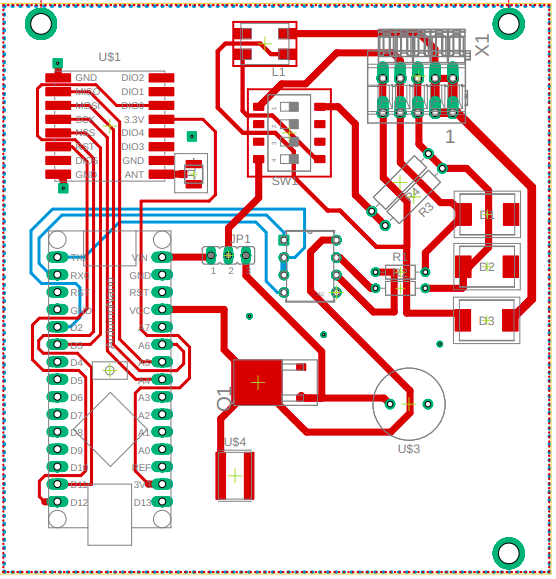
\includegraphics[width=0.7\textwidth]{minigateway_plosnak}
    \caption{Návrh \DIFdelbeginFL \DIFdelFL{WSN }\DIFdelendFL gatewaye verze 2 - plošný spoj}
    \label{fig:minigateway_plosnak}
\end{figure}
\DIFaddbegin 

\DIFadd{Použitý procesor neobsahuje paměť EEPROM, tudíž pro ukládání konfigurace gatewaye a zařízení senzorové sítě je použita paměť flash.
}\DIFaddend 



